\cleardoublepage
\chapter{HASIL PENGUJIAN}

Pengumpulan umpan balik dari partisipan dilakukan melalui dua pendekatan, yaitu kuantitatif dan kualitatif. Umpan balik kuantitatif digunakan untuk mengukur persepsi partisipan terhadap aspek-aspek sistem dalam skala numerik, sementara umpan balik kualitatif digunakan untuk menggali pengalaman subjektif dan saran perbaikan secara lebih mendalam. Data mentah responden dapat diakses melalui pranala \url{https://bit.ly/FeedbackTA-18222047}

\section{Umpan Balik Kuantitatif Pengujian}

\subsection{Daftar Pertanyaan Kuantitatif}
Berikut adalah daftar pertanyaan kuantitatif yang diajukan kepada partisipan:
\begin{enumerate}[1.]
    \item Selama sesi mengerjakan asesmen, seberapa sesuai kamu merasa tingkat kesulitan soal yang diberikan dengan kemampuanmu pada waktu tersebut? (Skala 0-5)
    \item Seberapa jauh kamu merasa kemampuanmu tentang SQL meningkat dibandingkan sebelum mengerjakan testing? (Skala 0-5)
    \item Apakah kamu merasa ada ``sense of community'' saat mengerjakan latihan soal dengan platform ini? (Skala 0-5)
    \item Sistem ini menggabungkan latihan yang dipersonalisasi dengan peer review, menurutmu apakah lebih baik sistem yang 100\% menyesuaikan soal SAJA (0) atau sistem yang seperti ini yang kadang ``memaksa'' kamu berinteraksi dengan rekan (5)? (Skala 0-5)
    \item Apakah ada momen saat kamu merasa ``stuck'' atau frustrasi karena tidak bisa unlock chapter selanjutnya? (Pilihan: Ya, Mungkin, Tidak)
    \item Sistem memberikan maksimum 3 kali percobaan (attempts) per soal. Apakah kamu merasa 3 kali cukup untuk belajar dari kesalahan? (Pilihan: Ya, Mungkin, Tidak)
    \item Apakah kamu merasa 3 kali percobaan tersebut terlalu sedikit atau terlalu banyak? (Pilihan: Terlalu Sedikit, Pas, Terlalu Banyak)
    \item Apakah kamu merasa tertekan dengan adanya batasan percobaan ini atau justru terbantu? (Pilihan: Tertekan, Terbantu)
    \item Apakah kamu merasa waktu 75 menit cukup untuk mengeksplorasi semua chapter materi? (Pilihan: Ya, Mungkin, Tidak)
\end{enumerate}

\subsection{Ringkasan Hasil Kuantitatif}
Hasil ringkasan statistik deskriptif dari data partisipan adalah sebagai berikut:

\begin{table}[!ht]
\centering
\caption{Statistik Deskriptif Metrik Utama Survei}
\label{tab:stats_deskriptif}
\begin{tabular}{l|c|c|c|c}
\hline
\textbf{Pertanyaan (Skala)} & \textbf{Mean} & \textbf{Std Dev} & \textbf{Min} & \textbf{Max} \\ \hline
Kesesuaian Kesulitan (0-5) & 4.10 & 0.32 & 4.00 & 5.00 \\
Peningkatan Kemampuan (0-5) & 4.60 & 0.52 & 4.00 & 5.00 \\
Sense of Community (0-5) & 3.20 & 1.23 & 1.00 & 5.00 \\
Preferensi Hybrid (0-5) & 3 & 1.67 & 0.00 & 5.00 \\ \hline
\end{tabular}
\end{table}


Ringkasan kategori untuk pertanyaan pilihan:
\begin{itemize}
    \item \textbf{Frustrasi/Stuck:} 80\% partisipan menjawab ``Ya'', menunjukkan tantangan pada ambang batas \textit{unlock} chapter.
    \item \textbf{Batas Percobaan (3x):} 50\% merasa ``Tertekan'' dan 50\% merasa ``Terbantu''. 40\% merasa jumlah percobaan tersebut ``Terlalu Sedikit''.
    \item \textbf{Kecukupan Waktu:} Mayoritas (80\%) merasa waktu 75 menit masih kurang untuk menyelesaikan seluruh materi.
\end{itemize}

\section{Umpan Balik Kualitatif Pengujian}

\subsection{Daftar Pertanyaan Kualitatif}
Berikut adalah daftar pertanyaan kualitatif terbuka yang diajukan:
\begin{enumerate}[1.]
    \item Jelaskan pengalamanmu mengenai adaptabilitas kesulitan soal dengan kemampuanmu.
    \item Jelaskan pengalamanmu mengenai ``sense of progression'' yang diberikan oleh sistem.
    \item Bagaimana pengalamanmu membaca perintah soal dan menggunakan editor SQL di platform ini? Apakah ada fitur yang kurang atau mengganggu?
    \item Jika dibandingkan dengan pengalaman menjawab soal praktikum/tugas SQL tradisional, apa yang lebih baik, lebih buruk, dan apakah kamu lebih memilih sistem ini?
    \item Apakah ada hal yang mengejutkan atau tidak kamu duga selama menggunakan sistem ini?
    \item Jika kamu bisa mengubah sistem ini, apa yang akan kamu ubah dan mengapa?
    \item \textit{(Grup Treatment)} Pengalaman memberikan feedback kepada teman (kesulitan memahami query, kebermanfaatan, keyakinan membantu).
    \item \textit{(Grup Treatment)} Pengalaman menerima feedback dari teman (pemahaman kesalahan, perbaikan cara berpikir, perbandingan dengan mencoba sendiri).
    \item Jelaskan alasan pemilihan angka pada skala preferensi sistem hybrid vs individual.
\end{enumerate}

\subsection{Ringkasan Hasil Kualitatif}
Ringkasan parafrasa dari jawaban partisipan adalah sebagai berikut:
\begin{itemize}
    \item Partisipan merasa sistem memberikan variasi soal yang baik, namun ada keluhan mengenai lonjakan kesulitan yang tiba-tiba (\textit{difficulty gap}) yang terkadang terasa tidak berjenjang.
    \item Keberadaan rating Elo memberikan efek ``reward'' dan ``punishment'' yang nyata. Namun, penurunan rating yang drastis saat gagal atau lambat mengerjakan soal dirasakan cukup ``kejam'' oleh beberapa partisipan.
    \item Antarmuka editor SQL yang berwarna dan memiliki \textit{auto-suggestion} sangat disukai. Namun, partisipan sangat mengharapkan adanya fitur \textit{run/preview query} sebelum melakukan submisi final.
    \item Feedback dari rekan dirasakan sangat membantu saat partisipan sudah benar-benar buntu (\textit{stuck}). Namun, ada keraguan mengenai kualitas feedback jika pemberi feedback sendiri belum menguasai materi tersebut.
    \item Sistem dinilai jauh lebih interaktif dan praktis dibandingkan metode praktikum tradisional karena integrasi materi, soal, dan lingkungan kerja dalam satu layar yang terstruktur.
\end{itemize}

\section{Data Mentah Peningkatan Hasil Belajar Individu}
\label{sec:lampiran_data_mentah}

Tabel \ref{tbl:nlg_individu} menyajikan data mentah performa belajar masing-masing partisipan secara individual selama sesi pengujian, yang mencakup kelompok, nilai praktikum, skor \textit{pre-test}, skor \textit{post-test}, serta perolehan \textit{Normalized Learning Gain} (NLG) teoretis dan empiris.

\begin{table}[!ht]
    \centering
    \caption{Data Mentah Hasil Belajar Individu Partisipan}
    \label{tbl:nlg_individu}
    \begin{tabular}{|p{2.0cm}|p{1.5cm}|p{1.8cm}|p{1.8cm}|p{1.8cm}|p{1.8cm}|p{1.8cm}|}
        \hline
        \textbf{Partisipan} & \textbf{Grup} & \textbf{Nilai Praktikum} & \textbf{Pre-test ($\theta$)} & \textbf{Post-test ($\theta$)} & \textbf{NLG Teoretis} & \textbf{NLG Empiris} \\
        \hline
        \hline
        User\_11 & A & 43,51 & 1260 & 1370,95 & 0,462 & 0,411 \\
        \hline
        User\_12 & A & 54,75 & 1340 & 1417,08 & 0,482 & 0,406 \\
        \hline
        User\_13 & A & 46,75 & 1420 & 1502,23 & 1,028 & 0,748 \\
        \hline
        User\_14 & A & 19,50 & 1260 & 1435,69 & 0,732 & 0,651 \\
        \hline
        User\_2  & A & 54,31 & 1260 & 1369,54 & 0,456 & 0,406 \\
        \hline
        User\_3  & A & 67,21 & 1340 & 1494,07 & 0,963 & 0,811 \\
        \hline
        \hline
        User\_1  & B & 44,81 & 1340 & 1376,50 & 0,228 & 0,192 \\
        \hline
        User\_5  & B & 35,25 & 1260 & 1030,65 & -0,956 & -0,849 \\
        \hline
        User\_6  & B & 44,16 & 1340 & 1325,64 & -0,090 & -0,076 \\
        \hline
        User\_9  & B & 59,62 & 1260 & 1253,80 & -0,026 & -0,023 \\
        \hline
    \end{tabular}
\end{table}

\section{Data Mentah Gradien \textit{Elo rating} (\textit{Slope}) Individu}
\label{sec:lampiran_data_slope}

Tabel \ref{tbl:slope_individu} menyajikan data mentah perubahan gradien \textit{elo rating} (\textit{slope}) untuk setiap partisipan sebelum dan sesudah intervensi, serta jumlah pemicuan stagnasi yang dialami selama sesi pengujian.

\begin{table}[!ht]
    \centering
    \caption{Data Mentah Gradien Kemahiran (\textit{Slope}) Sebelum dan Sesudah Pemicuan Stagnasi}
    \label{tbl:slope_individu}
    \begin{tabular}{|p{2.0cm}|p{1.8cm}|p{1.8cm}|p{1.8cm}|p{2.2cm}|p{2.2cm}|}
        \hline
        \textbf{Partisipan} & \textbf{Grup} & \textbf{Gradien Pre} & \textbf{Gradien Post} & \textbf{Perbedaan Gradien} & \textbf{Kejadian Stagnasi} \\
        \hline
        \hline
        User\_11 & A & -0,308 & 0,632 & 0,940 & 17 \\
        \hline
        User\_12 & A & -0,414 & -0,387 & 0,027 & 5 \\
        \hline
        User\_13 & A & 0,007 & 0,497 & 0,490 & 5 \\
        \hline
        User\_14 & A & -0,532 & 1,107 & 1,639 & 16 \\
        \hline
        User\_2  & A & -0,301 & 0,482 & 0,783 & 22 \\
        \hline
        User\_3  & A & 0,459 & 1,662 & 1,204 & 12 \\
        \hline
        \hline
        User\_1  & B & 0,039 & 0,078 & 0,040 & 17 \\
        \hline
        User\_5  & B & -0,835 & -0,791 & 0,045 & 38 \\
        \hline
        User\_6  & B & -0,168 & 0,081 & 0,248 & 15 \\
        \hline
        User\_9  & B & -0,084 & 4,668 & 4,752 & 31 \\
        \hline
    \end{tabular}
\end{table}


\section{Dokumentasi Pengujian}
Pengujian dilakukan di ITB. Gambar \ref{fig:dokumentasi_pengujian} menunjukkan dokumentasi pada saat pengujian dilakukan.

\begin{figure}[!ht]
    \centering
    \begin{subfigure}[b]{0.48\textwidth}
        \centering
        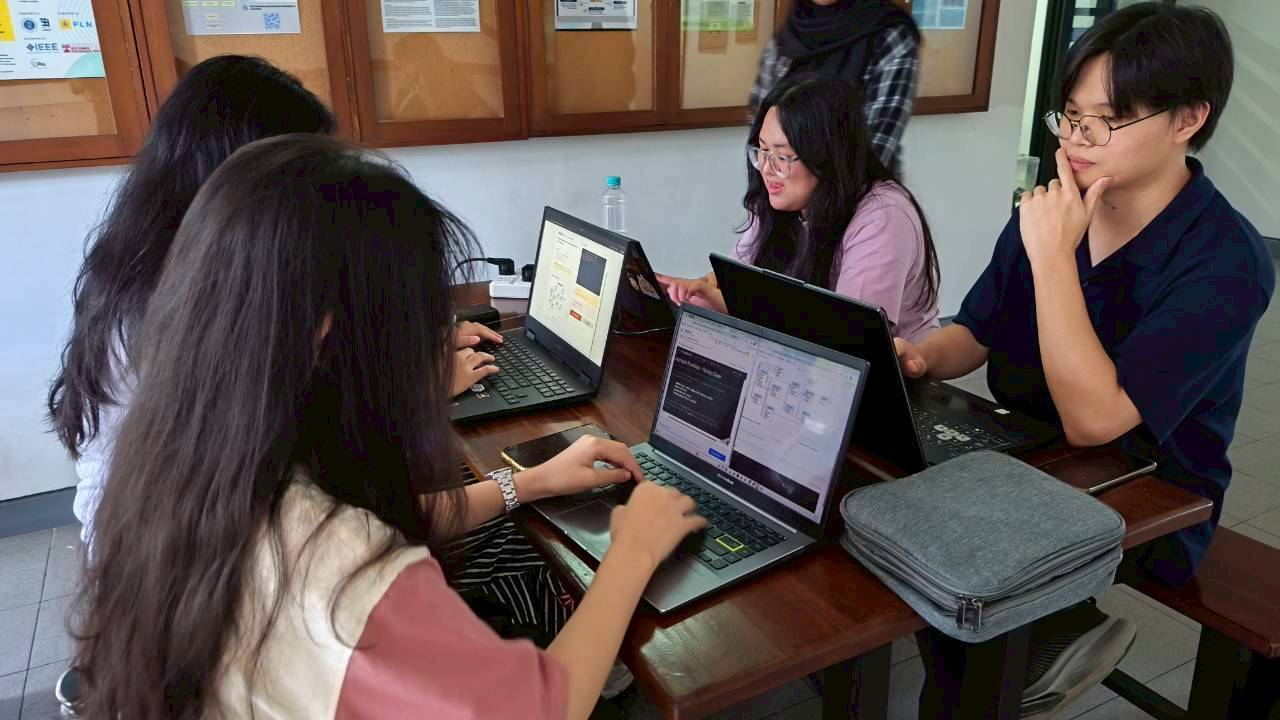
\includegraphics[width=\textwidth]{images/dokumentasi_pengujian_control_group.jpg}
        \caption{Sesi Pengujian Grup B (Kontrol)}
        \label{fig:dokumentasi_pengujian_control_group}
    \end{subfigure}
    \hfill
    \begin{subfigure}[b]{0.48\textwidth}
        \centering
        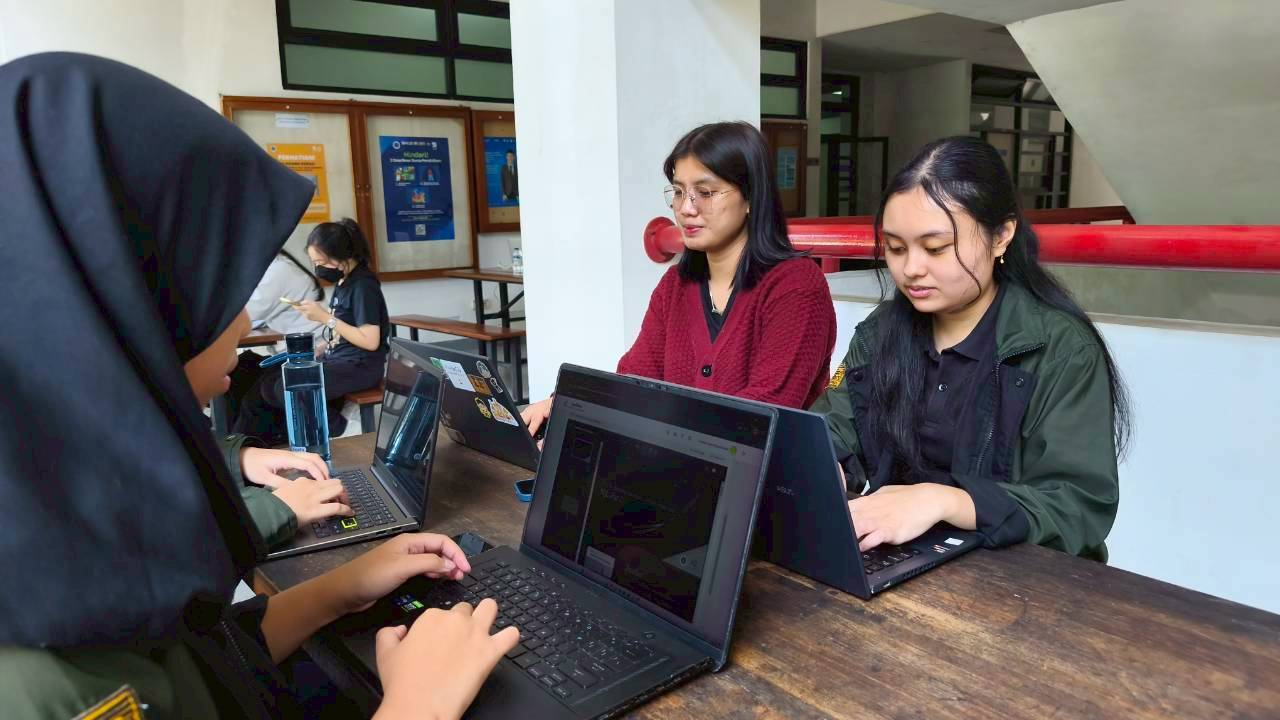
\includegraphics[width=\textwidth]{images/dokumentasi_pengujian_treatment_group.jpg}
        \caption{Sesi Pengujian Grup A (Treatment)}
        \label{fig:dokumentasi_pengujian_treatment_group}
    \end{subfigure}
    \caption{Dokumentasi Kegiatan Pengujian}
    \label{fig:dokumentasi_pengujian}
\end{figure}
